\chapter{Usage and experimentation} \label{chap:usage}

\section*{}

In this chapter is presented an usage example of the created prototype of this set of tools and methods. Is presented too a comparison between a manual evaluation and an evaluation generated by this tool.

\section{Usage example} \label{sec:usageexample}
	%Usage example - Dar um exemplo de utilização com printscrn

To demonstrate the prototype is presented in this section an usage example of the created methodologies and rules.

As said before all of this was implemented inside Scraim, so as a prerequisite is only possible to use this if you have an account on Scraim with this feature enabled.

\vspace{10 mm}

\textbf{Home Screen}

So if an user that is registered in Scraim is logged in his account, on the side bar of Scraim (its menu) is possible to see the assessment logo and if we click on that we will be guided to the assessments module homepage, presented in the Figure \ref{fig:no_assessments}.

\begin{figure}[h]
	\begin{center}
		\leavevmode
		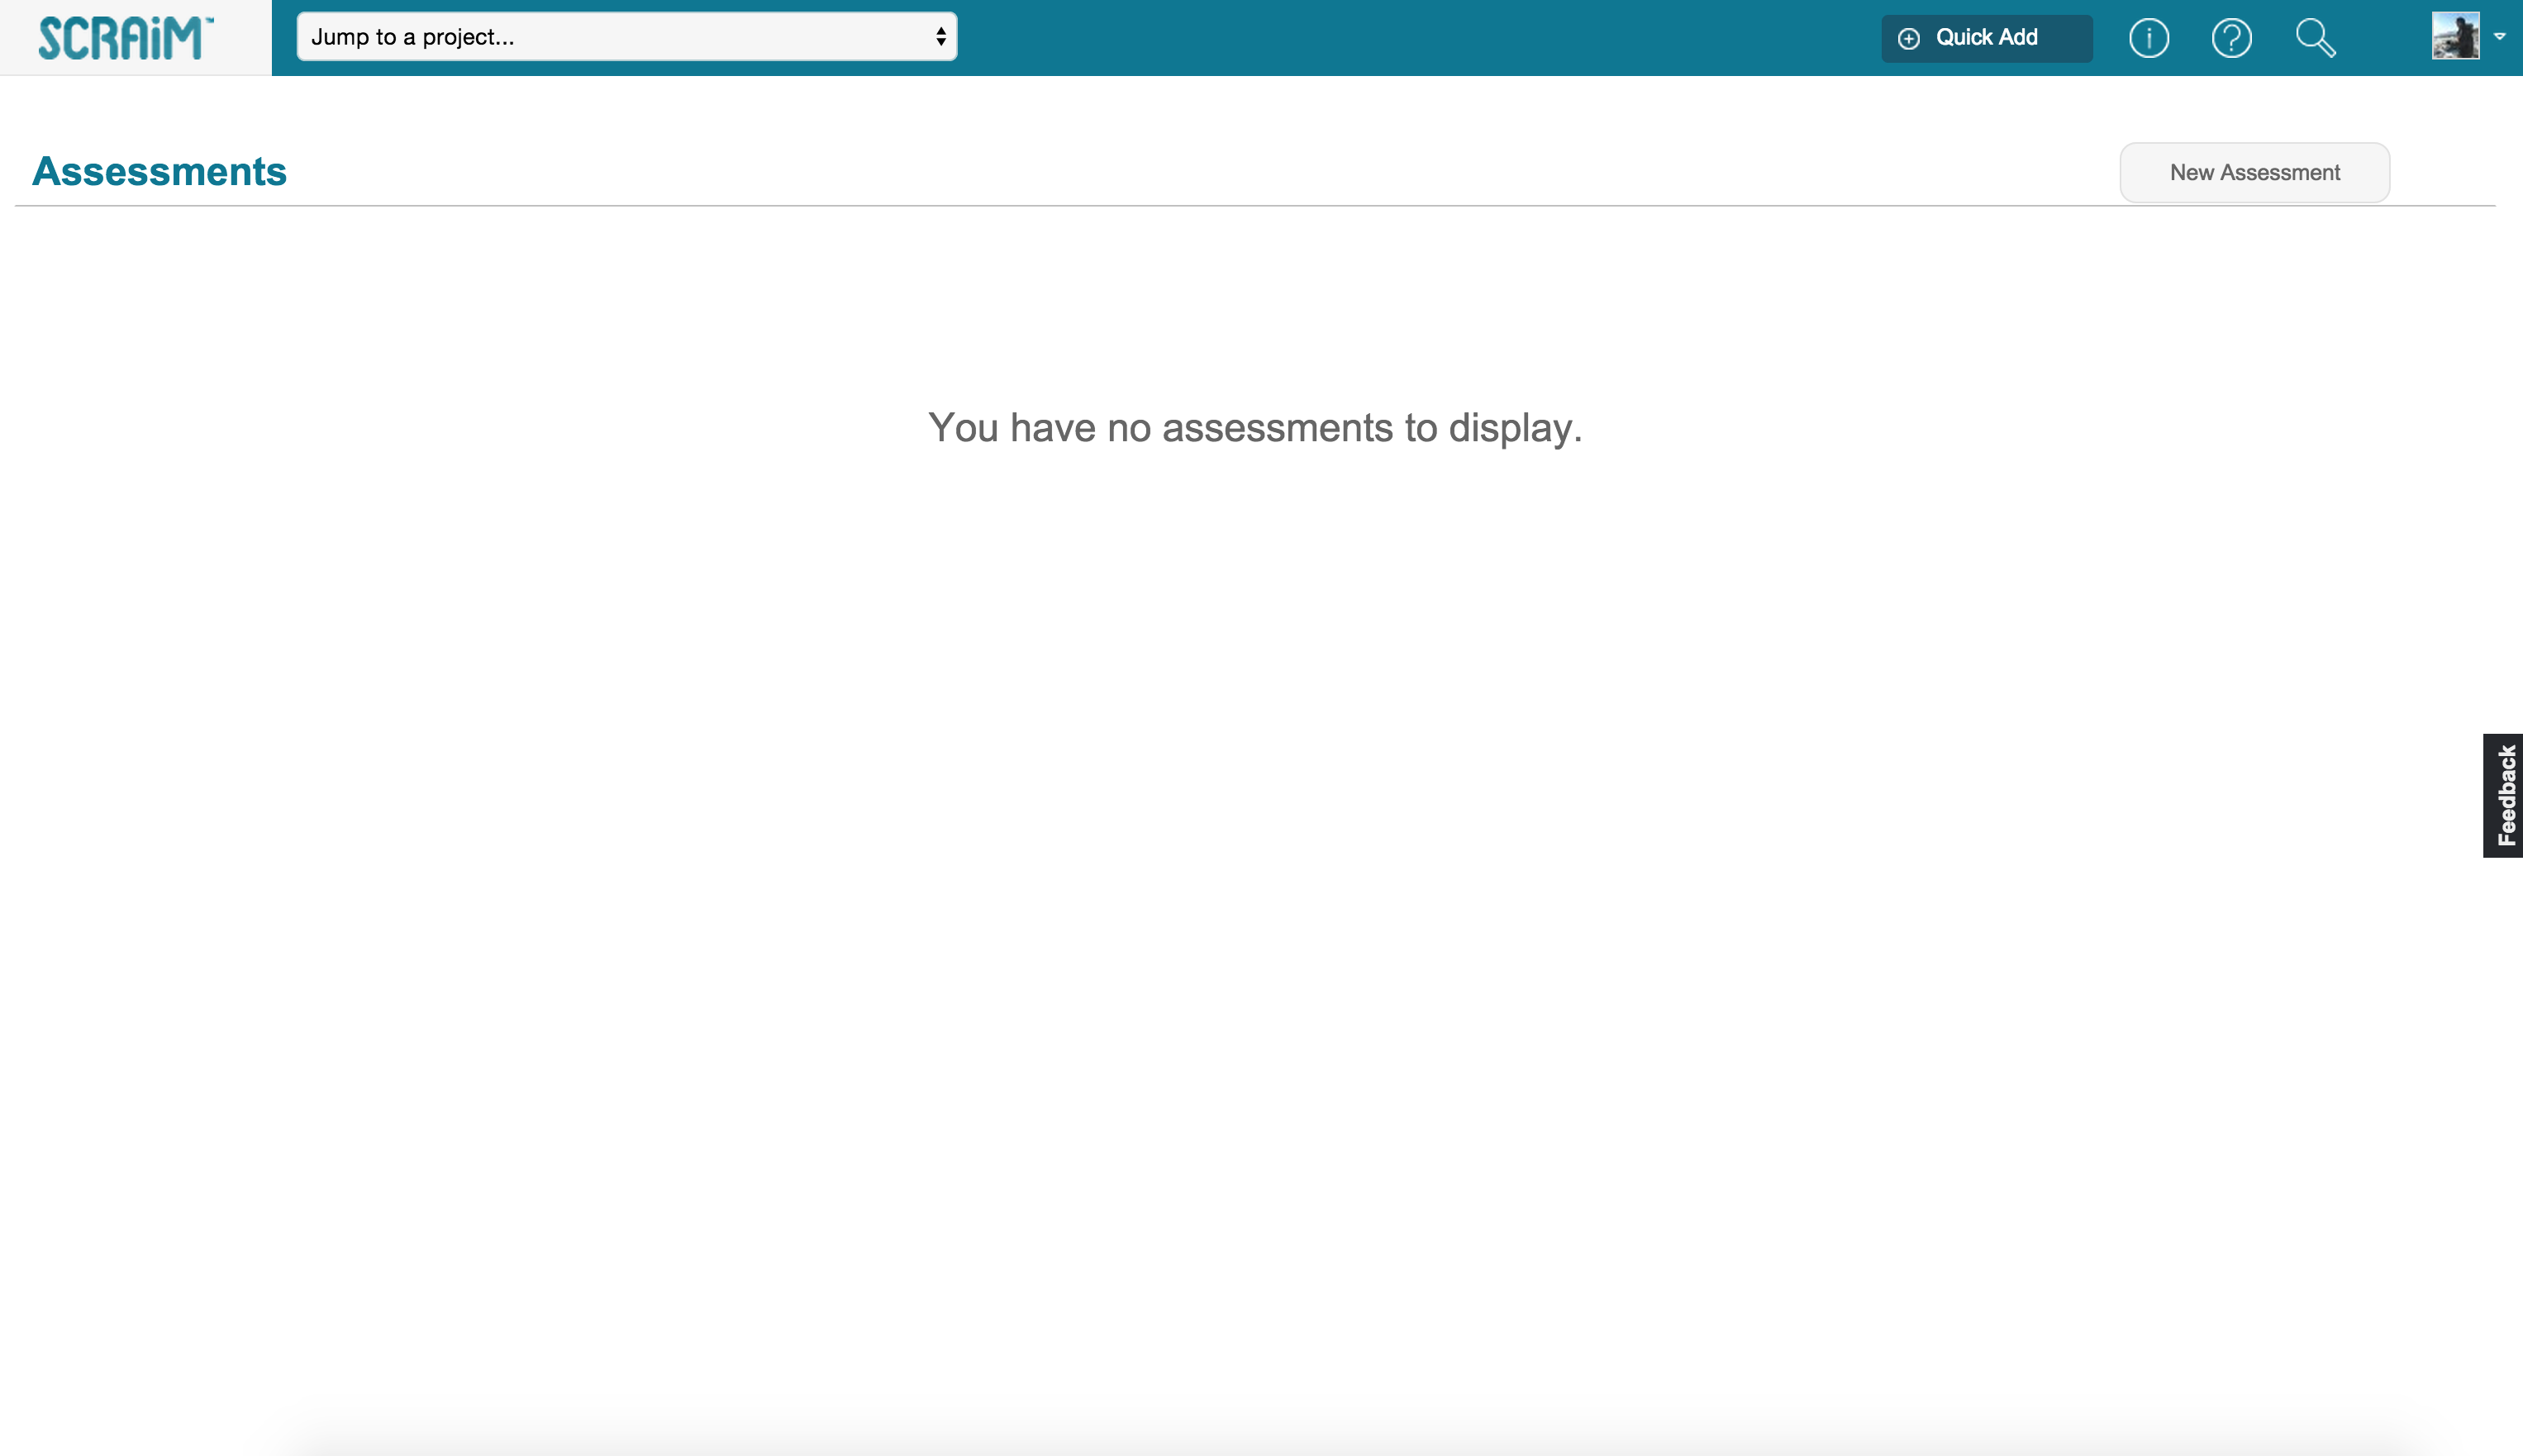
\includegraphics[width=0.9\textwidth]{no_assessments}
		\caption{Homepage without assessments done}
		\label{fig:no_assessments}
	\end{center}
\end{figure}

This screen is shown when we don't have assessments performed. If there are some done in this screen is presented a list of the assessments, like in the Figure \ref{fig:done_assessments}. In the Image, the three assessments are shown by ascending date order, so on bot are the most recent assessments.

\begin{figure}[h]
	\begin{center}
		\leavevmode
		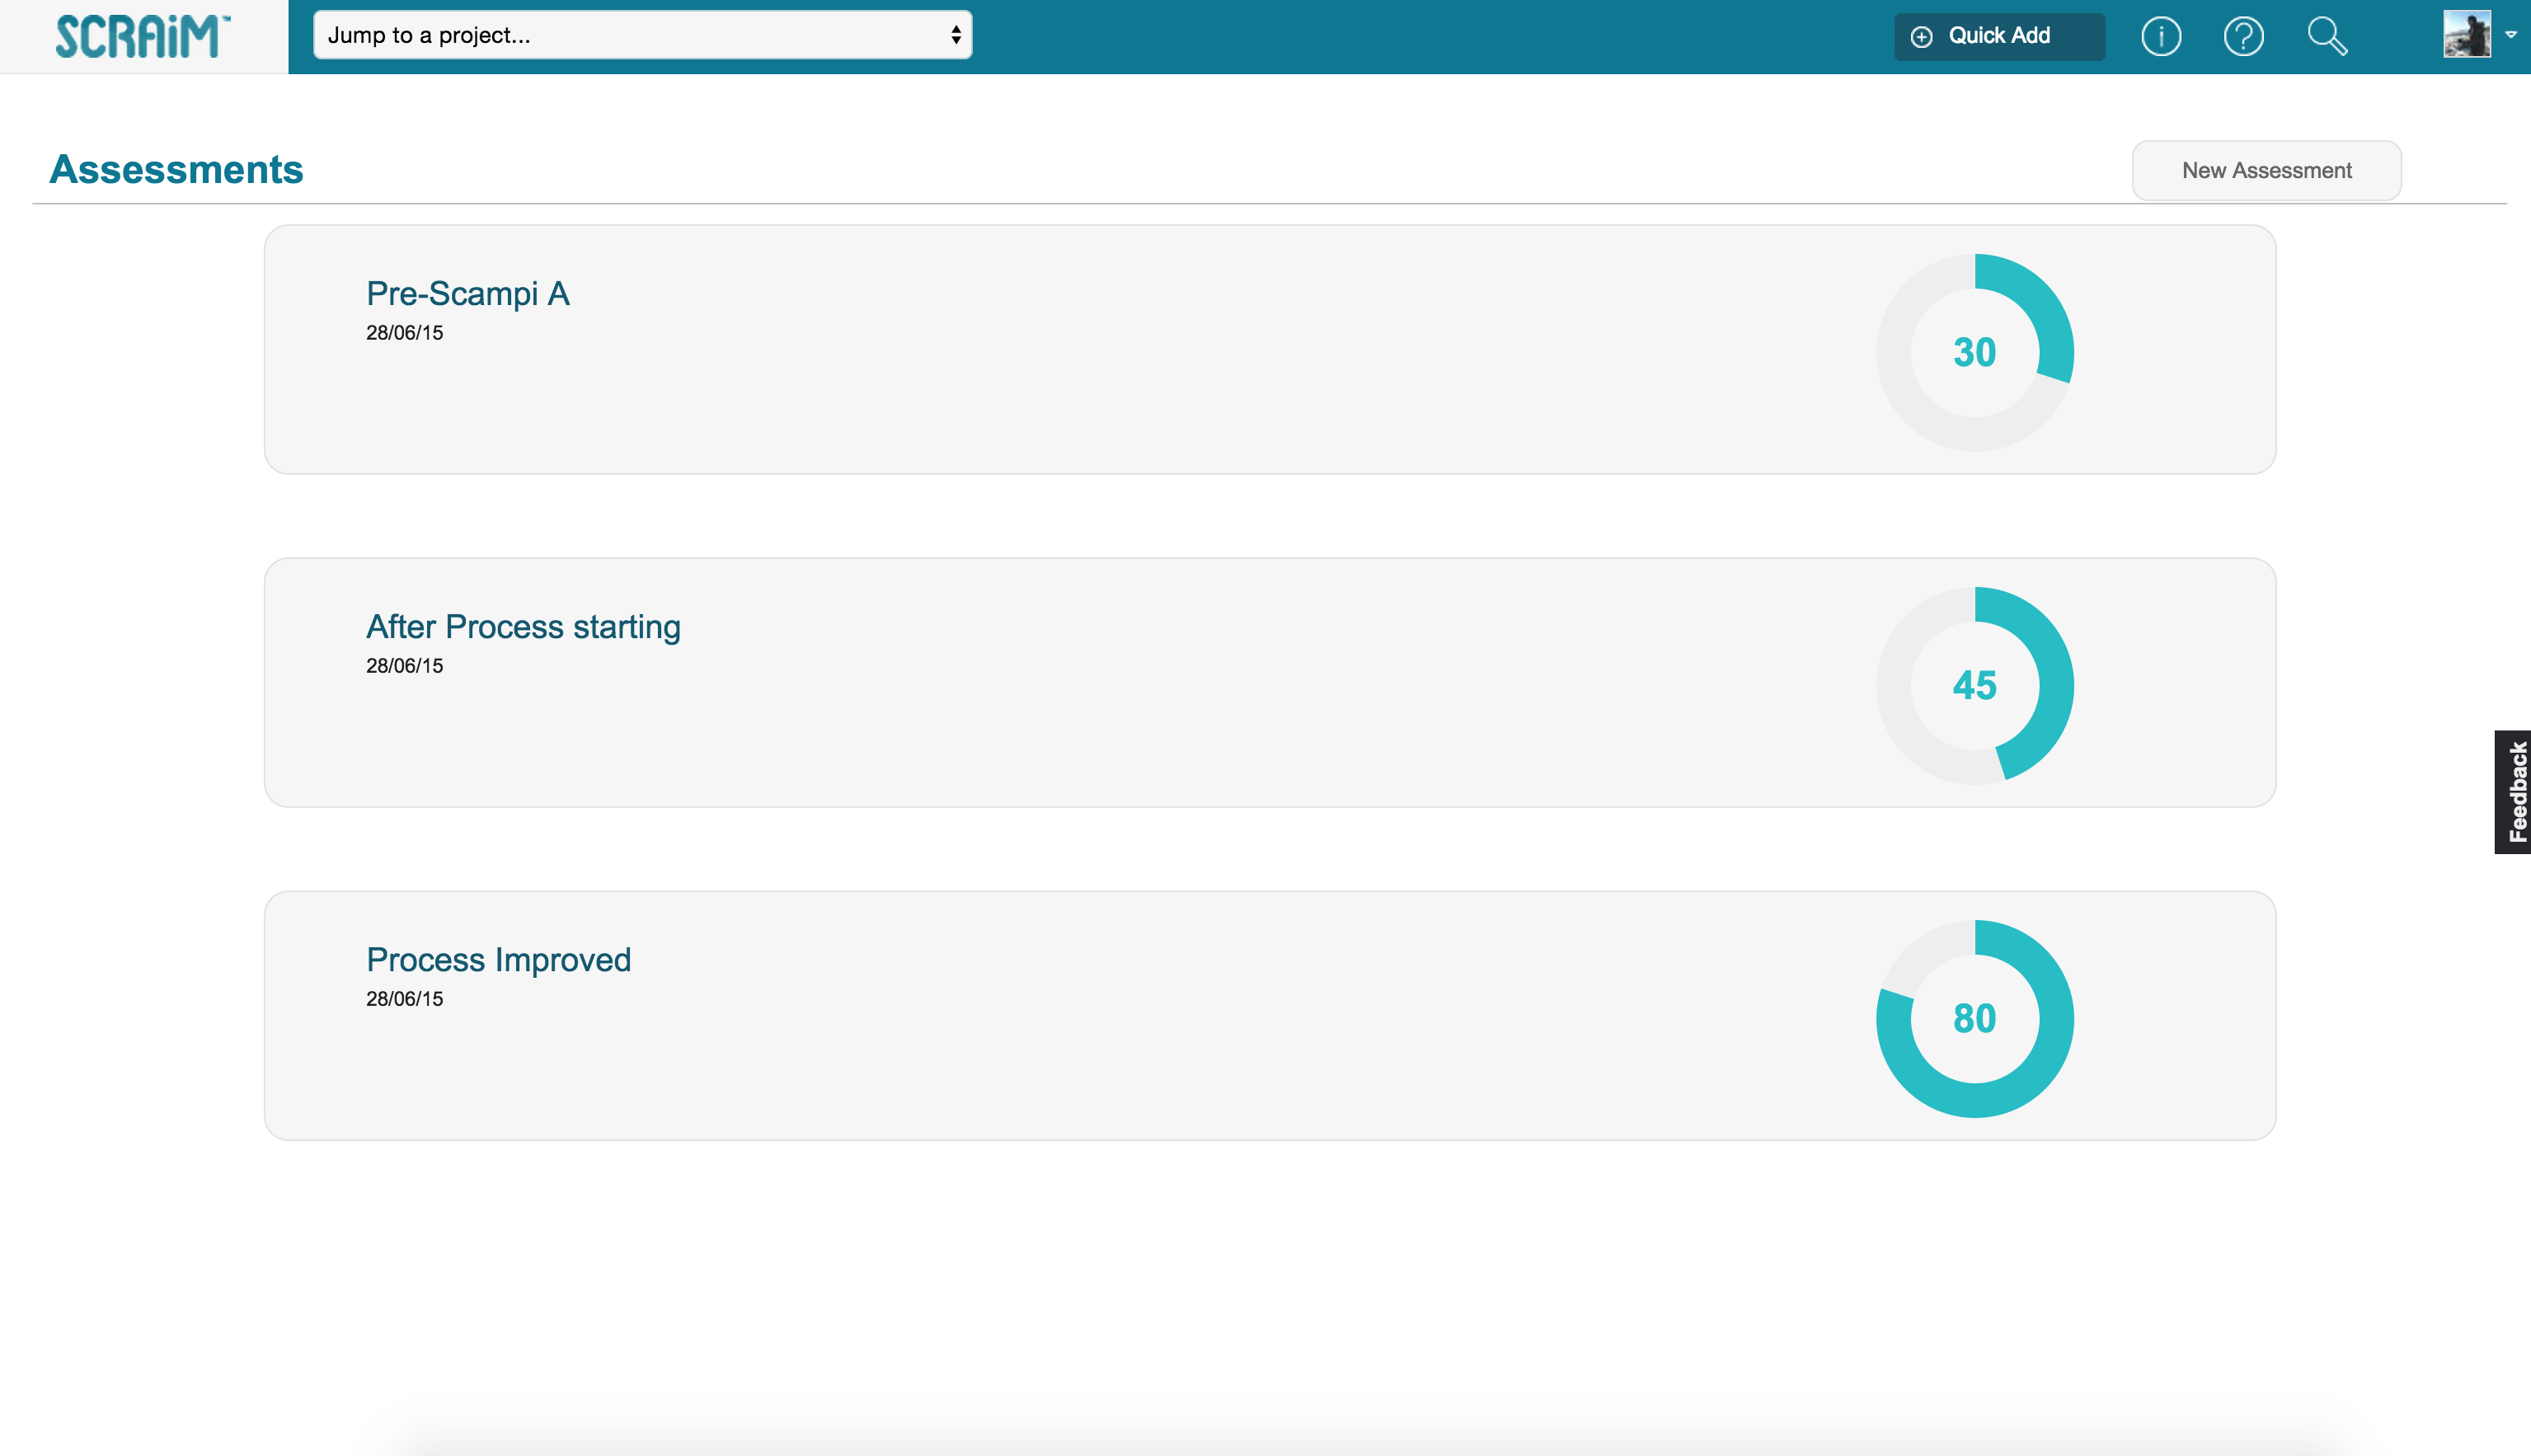
\includegraphics[width=0.9\textwidth]{done_assessments}
		\caption{Homepage with three assessments done}
		\label{fig:done_assessments}
	\end{center}
\end{figure}


\vspace{10 mm}

\textbf{Assessment Options}

In the Figure \ref{fig:done_assessments}, on the right top corner there is a button that says "New assessment". When that button is pressed the application leads us to a screen where is prepared the assessment. This preparation screen can be seen in the Figure \ref{fig:prepare_assessment}, in this page is needed to specify the name of the assessment if we want a custom name for the assessment. If the name is not specified a automatic name will be generated with the performed time and date of the assessment. Is needed too choose the project or projects that are going to be evaluated.

\begin{figure}[h]
	\begin{center}
		\leavevmode
		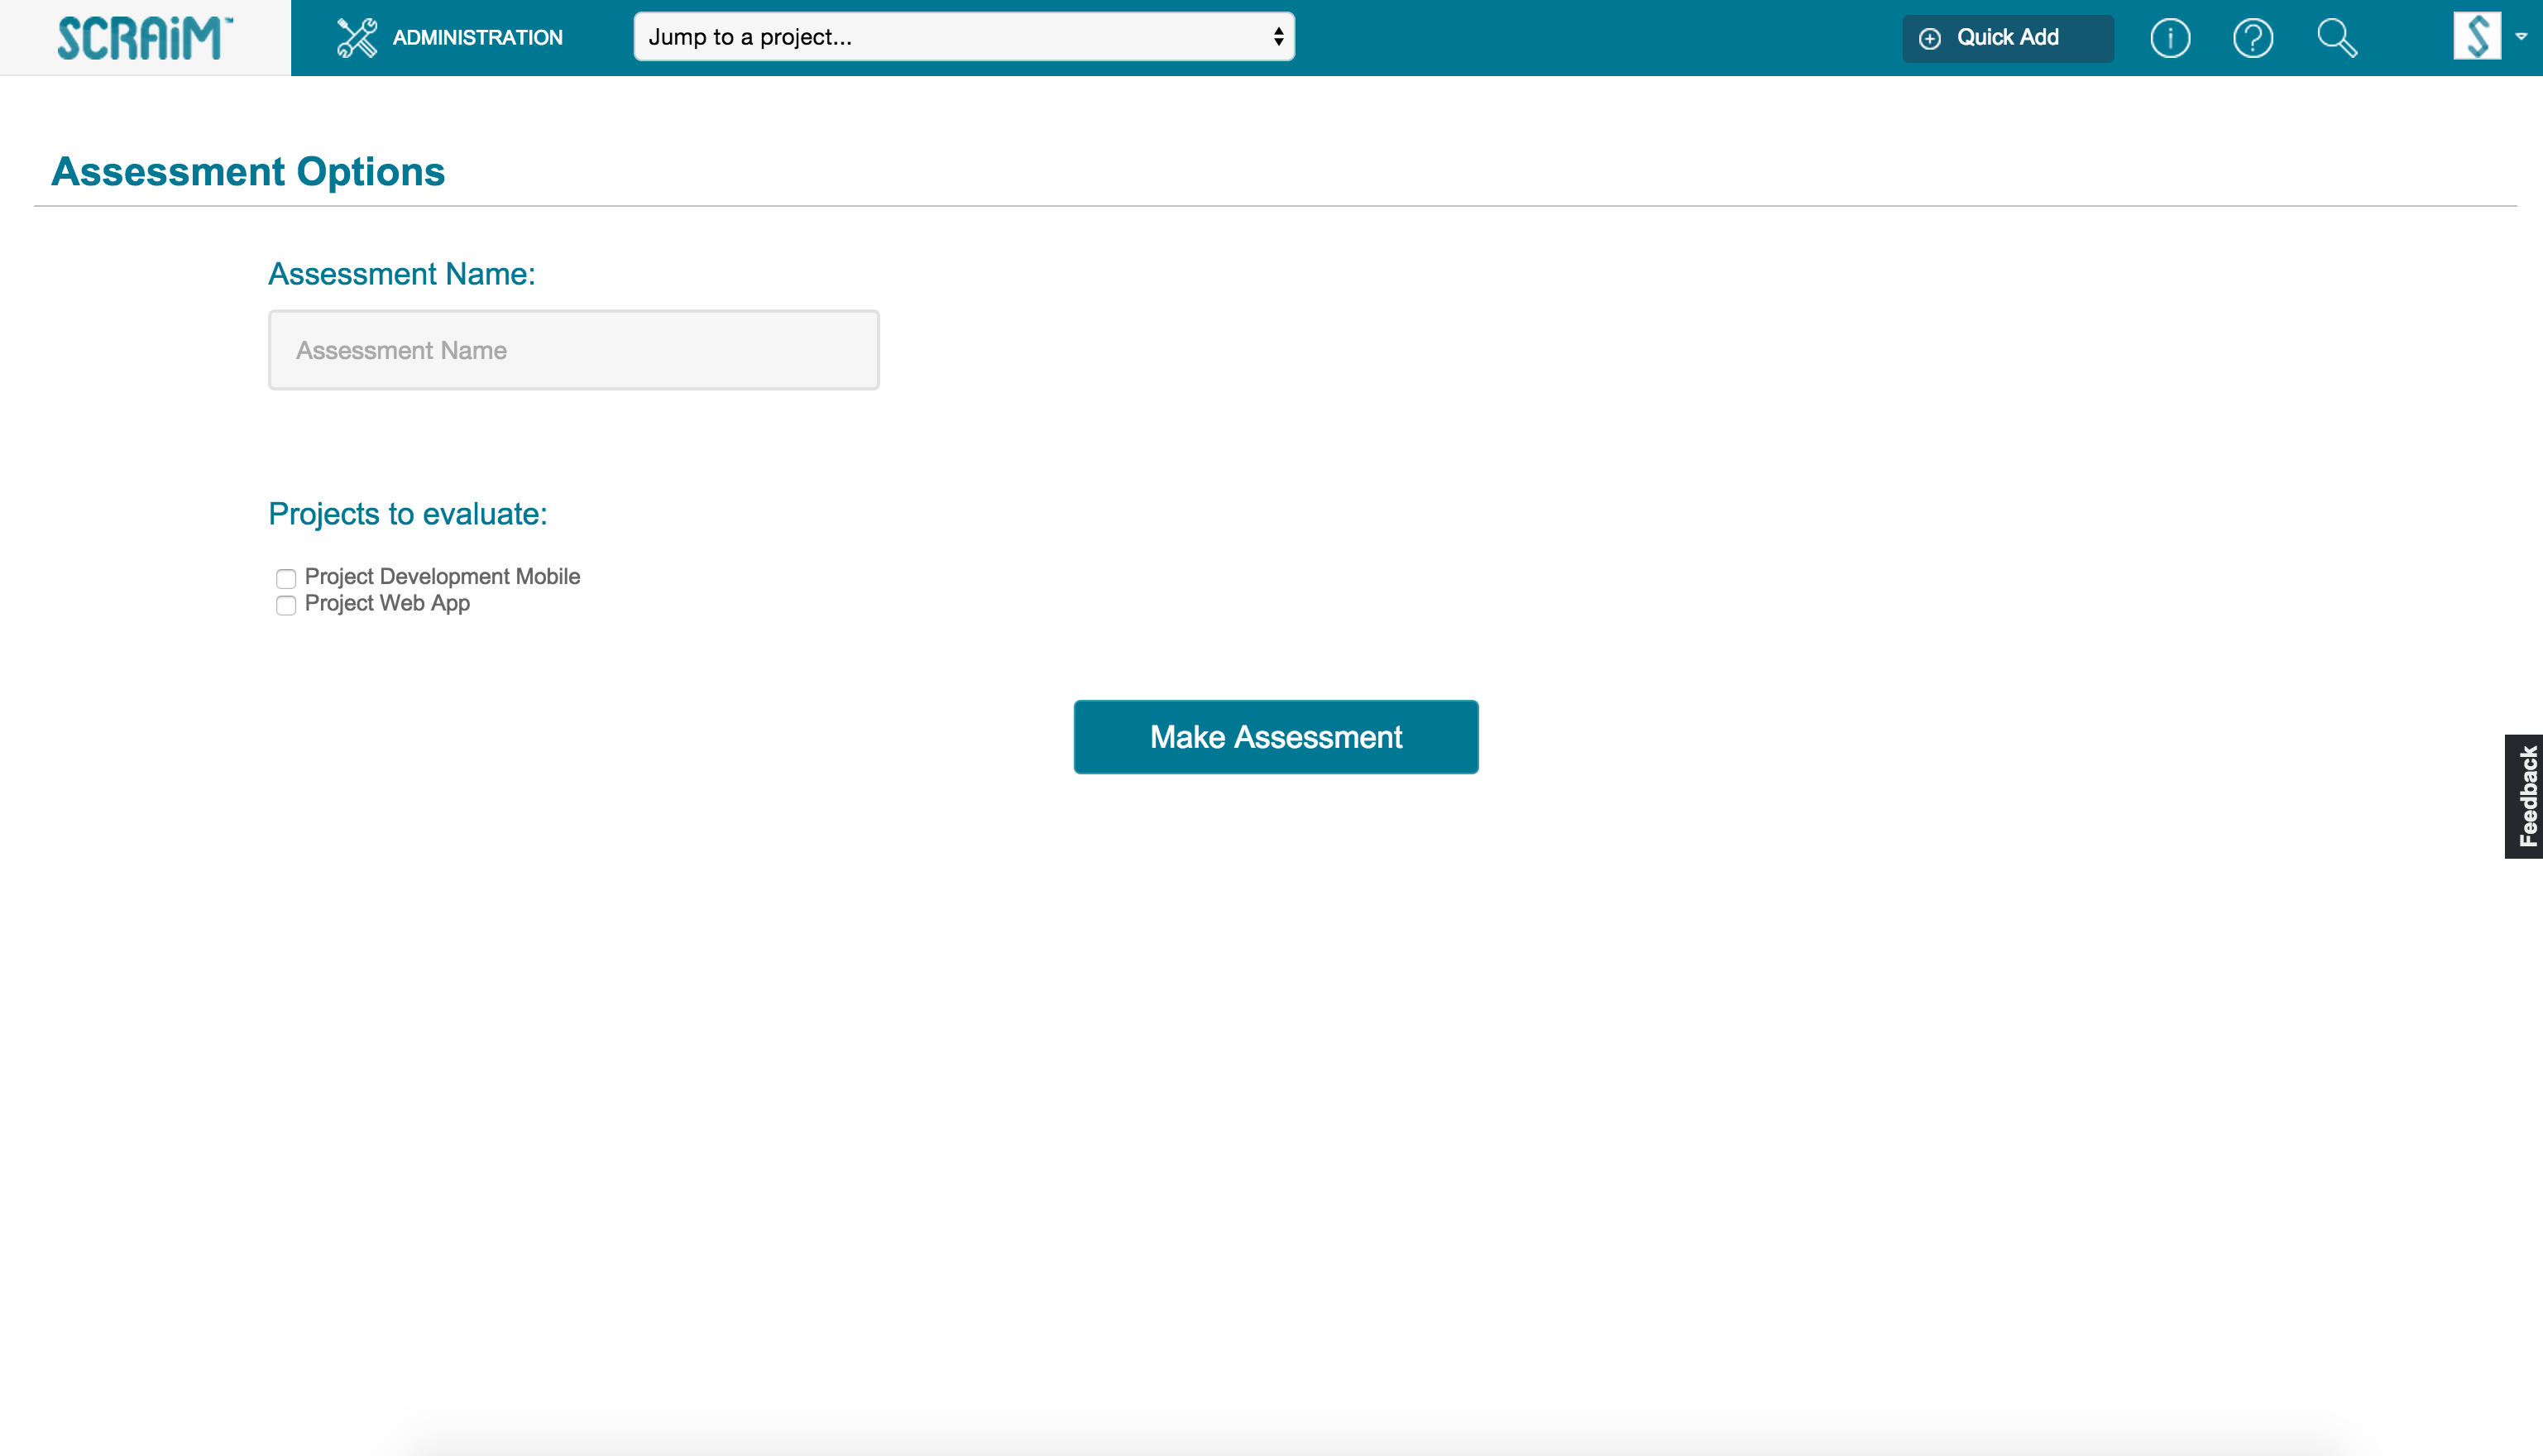
\includegraphics[width=0.9\textwidth]{prepare_assessment}
		\caption{Homepage without assessments done}
		\label{fig:prepare_assessment}
	\end{center}
\end{figure}

Only the text field can be empty, is mandatory to choose at least one project. After completing this process, the button make assessment can be clicked

Ecrã de passagem para o questionário

Ecrã mostragem de resultados

Inside resultados

Voltar à lista

\section{Coverage percentage} \label{sec:coverage}

%Scraim extension to increase cmmi coverage

Implementação até onde está neste momento falar das duas àreas totalmente implmentadas - PP e PMC
	
\section{Automatic vs Manual assessment} \label{sec:automatic}
%	Avaliação manual vs automatica

Aprensetntação da imagem de resultado final

Apresnetação da avaliação manual